\documentclass{scrreprt}

\usepackage{libertine}
\usepackage{graphicx}
\usepackage[table,xcdraw]{xcolor} %color in tables
\usepackage{hyperref}
\usepackage{array, tabularx, caption, boldline}
\usepackage{cellspace}
\usepackage{pdfpages} 
\usepackage{float}
\setlength\cellspacetoplimit{4pt}
\setlength\cellspacebottomlimit{4pt}
\usepackage{tikz}
\newcommand*\circled[1]{\tikz[baseline=(char.base)]{
		\node[shape=circle,draw,inner sep=2pt] (char) {#1};}}

\RedeclareSectionCommand[
  beforeskip=-.5\baselineskip,
  afterskip=.25\baselineskip]{subsubsection}
\RedeclareSectionCommand[
  beforeskip=-.5\baselineskip,
  afterskip=-0.5em]{paragraph}
\RedeclareSectionCommand[
  beforeskip=-.2\baselineskip,
  afterskip=-0.5em]{subparagraph}

\subject{EP Secure Cloud Energy Monitoring Platform WS 2018/19}
\title{Design}
\subtitle{Scrum Master and Product Owner: Andreas M\"uller}
\author{Martin Binder\\Korbinian Simonis\\Benedikt Holler\\Andreas M\"uller\\Simon Sch\"onberger}
\date{As of \today}
\dedication{
  {\titlefont \LARGE Hello there!}\\
  We're Team Hams and we're doing our very best to deliver only the finest software.\\~\\
  
\includegraphics{team-normal.jpeg}
}

\begin{document}
\maketitle
\tableofcontents
%----------------------------------------------%
\chapter{Use Case}
%-----------------------------%
\section{User Specification}
Author: Benedikt Holler | Reviewer: Korbinian Simonis \\ \\
We have defined three types of users that have access to the EMS. Each of them has different rights, which will briefly be summarized here. \\
Privileged Users have all Regular User Rights; likewise, all Administrators have all Privileged User Rights and Regular User Rights. 
\subsection{Regular User Rights}
\paragraph{Reading Node Information.}
Displaying all information regarding nodes the user has access to. This includes node name, KPI units and values, and whether a node is estimating KPIs.
\paragraph{Configuring Alert Rules.} 
For each node they have access to, the user can set up Alert Rules. These include a name, description, KPI thresholds, and settings for Oscillation Handling.
\subsection{Privileged User Rights}
\paragraph{Managing User Groups.}
Users can only view nodes if they are a member of an User Group, and only if that group has access to those nodes. Privileged Users act as supervisors for User Groups. They can edit group information and manage user memberships, i.e. adding and removing users from groups. 
\paragraph{Changing Node Sent Intervals.}
Privileged Users also have the ability to change the interval in which nodes send KPI values to the Backend server. However, they can only change this setting on nodes which are assigned to groups they manage.
\subsection{Administrator Rights}
\paragraph{User Management.} Administrators are able to create and delete users, and can edit user information.
\paragraph{User Group Management.} Only administrators can create new User Groups, delete them, and assign nodes to groups.
\paragraph{Node Management.} An Administrator can change certain aspects of nodes, such as changing the name. However, they can explicitly not change internal settings of the Monitoring Client, such as the way that KPI data is aggregated.
\section{Use Case Diagram}
Author: Martin Binder | Reviewer: Andreas M\"uller
\begin{figure}[h!]
	\includegraphics[width=\linewidth]{uml/usecasediagram1.pdf}
	\caption{Simplified view Use Case}
	\label{usecase1}
\end{figure}	
%-----------------------------%
\section{Use Case}
Author: Teamwork \\ \\
%this is our template for the use cases.
%linebreaks are performed automatically if you reached the max width of a cell.
%if you need to force a linebreak within a cell use the \newline command.
Prerequisites to use the HAMer Tool and not explicitly mentioned in every Use Case: \\
- Access to the Intranet on which HAMer is deployed.\\
- A compatible Browser (i.e. Firefox or Chrome). \\
- The Frontend is up and reachable.
- The Backend is up and reachable. \\
\\
\\ \\
\begin{tabularx}{12cm}{l|X}
ID & UC01  \\
\hline
Label & 
A User logs in on the EMS website. \\
\hline
Actor            & User    \\
\hline
Description            &  	1. User enters their user name. 2. User enters their password. 3. User clicks on "Login". 4. System authorizes User to access the EMS. \\
\hline
Precondition           &   User has a valid account.\\ 
\hline
Postcondition     & User is logged into the system and accesses the content. \\
\hline
Exceptional Cases & 1. User has no account. 2. User enters wrong password. 3. User enters wrong user name. 
4. System can't process request.
\end{tabularx}
\\
\\ \\
\begin{tabularx}{12cm}{l|X}
ID & UC02  \\
\hline
Label & 
A User logs out. \\
\hline
Actor            & User   \\
\hline
Description            &  	1. User clicks log out. 2. System destroys user session.  \\
\hline
Precondition           &   User is logged in.\\ 
\hline
Postcondition     & User is logged out and can't access EMS without re-authentication. User session is destroyed. \\
\hline
Exceptional Cases & 1. System can't process request.
\end{tabularx}
\\
\\ \\ 
\begin{tabularx}{12cm}{l|X}
ID & UC03  \\
\hline
Label & 
Evaluate KPIs. \\
\hline
Actor            & User   \\
\hline
Description            &  	1. User accesses the Dashboard.	
2. User sees Overview of energy consumption of all supervised nodes. 3. User picks a specific node. 4. User picks a specific KPI. 5. User enters date and time period. 5. System provides visualized data for the entered conditions.
\\
\hline
Precondition           & 1. User has a valid account. 2. User performs a successful login. 3. KPIs exist for the picked time frame.  \\
\hline
Postcondition     & System provides specific data on the picked KPI in a certain time frame. \\
\hline
Exceptional Cases & 1. KPIs don't exist. 2. System can't process request.
\end{tabularx}
\\
\\ \\ 
\begin{tabularx}{12cm}{l|X}
ID & UC04  \\
\hline
Label & 
A User edits their profile. \\
\hline
Actor            & User    \\
\hline
Description            &  	1. User clicks on "Edit Profile" on the Navigation Bar on the left side of the screen. 2. System redirects User to the Edit Profile page. 3. User edits their profile (e-mail, password etc.) 4. System saves changes on the Users profile.   
\\
\hline
Precondition           & 1. User has a valid account. 2. User is logged in.  \\
\hline
Postcondition     & BE processes the changes and updates the database. \\
\hline
Exceptional Cases & 1. Input is invalid. 2. System can't process request.
\end{tabularx}
\\
\\ \\
\begin{tabularx}{12cm}{l|X}
ID & UC05  \\
\hline
Label & 
User sets their Alert Notification. \\
\hline
Actor            & User  \\
\hline
Description            &  	1. User clicks on "Alert Notification" on the Navigation Bar on the left side of the screen. 2. System redirects User to the Alert Notifications page. 3. User creates an alert notification. 4. User assigns alert notification to nodes. 5. User clicks on "Save changes" 6. System saves changes.   
\\
\hline
Precondition           & 1. User has a valid account. 2. User is logged in.   \\
\hline
Postcondition     &  New alert notification is in database. 2. Alert notification is assigned to nodes. \\
\hline
Exceptional Cases & 1. Input is invalid. 2. System can't process request.
\end{tabularx}
\\
\\ \\ 
\begin{tabularx}{12cm}{l|X}
ID & UC06  \\
\hline
Label & 
An Administrator manages user accounts. \\
\hline
Actor            & Administrator   \\
\hline
Description            &  	1. Administrator clicks on "User Management" on the Navigation Bar on the left side of the screen. 2. System redirects Administrator to the User Management page. 3. Administrator manages user profile. 4. System saves changes on the Users profile.   
\\
\hline
Precondition           & 1. Administrator has a valid account. 2. Administrator is logged in.  \\
\hline
Postcondition     & BE processes the changes and updates the database. \\
\hline
Exceptional Cases & 1. Input is invalid. 2. System can't process request.
\end{tabularx}
\\
\\ \\
\begin{tabularx}{12cm}{l|X}
ID & UC07  \\
\hline
Label & 
An Administrator manages user groups. \\
\hline
Actor            & Administrator    \\
\hline
Description            &  	1. Administrator clicks on "Group Management" on the Navigation Bar on the left side of the screen. 2. System redirects Administrator to the group management page. 3. Administrator manages user groups. 4. Administrator clicks on "Save changes". 5. System saves changes.  
\\
\hline
Precondition           & 1.Administrator has a valid account. 2. Administrator is logged in.  \\
\hline
Postcondition     & BE processes the changes and updates the database.\\
\hline
Exceptional Cases & 1. Input is invalid. 2. System can't process request.
\end{tabularx}
\\
\\ \\
\begin{tabularx}{12cm}{l|X}
ID & UC08  \\
\hline
Label & 
A Privileged User manages nodes. \\
\hline
Actor            & Administrator, Privileged User    \\
\hline
Description            &  	1. Privileged User clicks on "Node Management" on the Navigation Bar on the left side of the screen. 2. System redirects Privileged User to the node management page. 3. Privileged User manages nodes. 4. Privileged User clicks on "Save changes". 5. System saves changes.  
\\
\hline
Precondition           & 1.Privileged User has a valid account. 2. Privileged User is logged in.  \\
\hline
Postcondition     &  BE processes the changes and updates the database.\\
\hline
Exceptional Cases & 1. Input is invalid. 2. System can't process request.
\end{tabularx}
\\
\\ \\
\begin{tabularx}{12cm}{l|X}
ID & UC09  \\
\hline
Label & 
A privileged User manages user groups. \\
\hline
Actor            & Privileged User    \\
\hline
Description            &  1. Privileged User clicks on "Group Management" on the Navigation Bar on the left side of the screen. 2. System redirects privileged User to the group management page. 3. Privileged User manages user groups. 4. Privileged User clicks on "Save changes". 5. System saves changes. 
\\
\hline
Precondition           & 1.Privileged User has a valid account. 2. Privileged User is logged in.  \\
\hline
Postcondition     &  BE processes the changes and updates the database. \\
\hline
Exceptional Cases & 1. Input is invalid. 2. System can't process request. 	
\end{tabularx}
\\
\\ \\
\begin{tabularx}{12cm}{l|X}
	ID & UC10  \\
	\hline
	Label & 
	A Node provides KPI data. \\
	\hline
	Actor            & Node    \\
	\hline
	Description            &  1. Node installs MC. 2. Node registers to BE. 3. Node collects KPIs. 4. Node sends KPIs to BE.
	\\
	\hline
	Precondition           & 1. Node has a valid token. 2. Node is registered at BE  \\
	\hline
	Postcondition     &  BE receives KPIs from Node and stores them in database. \\
	\hline
	Exceptional Cases & 1. KPIs are accessible. 2. BE is reachable. 	
\end{tabularx}
\\
\\ \\
% ----------------------------------------- %
\section{User Story}
Author: Teamwork
\subsection{INVEST Principle}
The User stories follow the \textbf{INVEST} principle. To count as a User Story the following requirements have to be met: 
\paragraph{I = Independent} User Stories can't be dependent on other User Stories. If that's the case the Story has to be split up, written in a more generic way or if that's not possible, dropped.
\paragraph{N = Negotiable} The term negotiable means that User Stories have to leave some room for changes if necessary.
\paragraph{V = Value} They increase the product value. 
\paragraph{E = Estimate-able} The cost of implementation is estimate-able if a User Story can't be estimated in a foreseeable way it has to be dropped.
\paragraph{S = Small} The User Stories are as small as possible and split down into an atomic form if doable.
\paragraph{T = Testable} The outcome can be tested. If the outcome is vague, the User Story has to be dropped.  \\
\subsection{Stage names:}
Each User Story bears the avatar of one team member. This is the list of their allocation. \\ 
\begin{tabularx}{8cm}{l|l}
	Martin Binder & \textbf{Cool Cat} \\
	Korbinian Simonis & \textbf{Snoop Dog} \\
	Benedikt Holler & \textbf{Nite Owl III.} \\
	 Andreas M\"uller & \textbf{Spooky Ghost} \\
	 Simon Sch\"oenberger & \textbf{Bearded Lumberjack} 
\end{tabularx}

	\includepdf[width=15cm, pages={1},pagecommand={\subsection{User Stories, JIRA Export}}]{backlog/s03_hams_productbacklog_export.pdf}
	\label{userstory1}
	
	\includepdf[width=15cm, pages={2-}]{backlog/s03_hams_productbacklog_export.pdf}
	\label{userstory}
\chapter{System Architecture}
% ================================================================ %
Author: Simon Sch\"onberer | Reviewer: Martin Binder\\ \\
Our system consists of three parts: Frontend (FE) for user interaction through a reactive, 
modern single-page-application, a Backend (BE) which provides core features like data processing,
persistence etc., and Monitoring Clients (MC) which are installed on the nodes in order to
gather KPIs for further evaluation. Figure \ref{sys-comp} gives an overview.

\begin{figure}[h]
	\centering
	\includegraphics[width=\linewidth]{architecture/s03_hams_components.pdf}
	\caption{Component architecture of our MEMS.}
	\label{sys-comp}
\end{figure}

\section{Frontend}
% ----------------------------------------- %
Author: Simon Sch\"onberer | Reviewer: Martin Binder
\subsection{Technologies}
Author: Benedikt Holler | Reviewer: Martin Binder
\paragraph{Nuxt.js.} Nuxt.js offers the benefits of vue.js as a UI-rendering, feature-rich frontend framework with the advantages of Vue2, Vue Router, Vue Server Renderer, Vue meta as well as the webpack + vue loader and babel loader to enable Javascript ES6 and ES7. \\
Additionally, nuxt.js comes with a project structure by default (components, layouts, pages, store) which supports building flexible, reactive Single Page Applications efficiently and develop a User friendly Web-application. 
\paragraph{Chart.js} Since data representation is the core functionality and task of the HAMerEms, charts are a critical feature of our frontend interface, thus developing precise, meaningful, easy to understand and good looking charts is indispensable. Chart.js offers great implementation of many different chart types which suit the needs of the data represented. Additionally, chart.js offers highly configurable utilization of data representation which is essential for a successful design.
\subsection{Architecture}
\paragraph{MVVM.} Vue.js provides the architectural core of the Frontend. It is a \emph{MVVM}
framework which supports building MVVM-based SPAs. Therefore our Frontend application will be
heavily based on the MVVM pattern.
\\ \\ 	
\begin{figure}[h]
	\centering
	\includegraphics[width=12cm]{architecture/mvvm-architecture.pdf}
	\caption{Navigation flow state chart}
	\label{MVVM}
\end{figure}
\\
On a low-level view, each component will use vue's component-based approach to develop
reusable components that each consist of \emph{View} and \emph{ViewModel}. They will be bound
to the model via a nuxt.js helper called \emph{asyncData}, but anyway, the model consists 
just of asynchronous HTTP-calls or incoming STOMP-updates. Vue.js takes
care of data binding between View and ViewModel, to make them independent of one another.
Note that vue keeps things simple by reducing data binding to the lowest possible level, and therefore only enables single-way-bindings by default. By using the dedicated
API functions provided, two-way-bindings can be easily accomplished and will be used in our
application wherever it adds value.
On a higher level, many components will be put together to build the application. Those components
can be roughly divided into three categories, according to the structure nuxt leverages:
\emph{Pages}, \emph{(reusable) Components} and \emph{Layouts}.
Layouts define template-like structures, where the route-dependent content can be wrapped in.
Pages will provide a logical unit of the applications interfaces, even in terms of routing.
They will represent a view or part of a view like e.g. "Dashboard".
Last but not least, Components build small, heavily reusable units which implement widely used
functions like single buttons, text inputs, etc.
\emph{Maybe merge this with "Components" and go on writing about the definitive components here.}
\subsection{Views}
Author:  Andreas M\"uller | Reviewer: Benedikt Holler\\
\paragraph{Login.} The login view queries the user for credentials which shall be submitted
consequently. If the credentials entered are valid, the user will be forwarded to the dashboardConfiguration,
otherwise an error message will be added to the login view e.g. "Forgot Password?". The login view comes with the 'blank'
layout. See Figure \ref{login} for a prototype.
\begin{figure}[h]
  \centering
  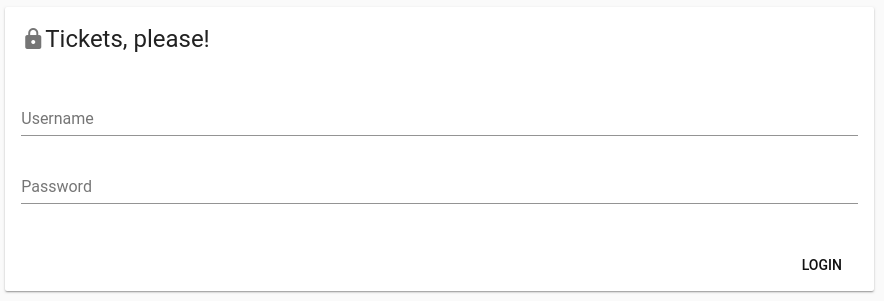
\includegraphics[width=.7\linewidth]{prototype/login}
  \caption{Prototype of the login page.}
  \label{login}
\end{figure}
%-------------------------------------------%
\paragraph{Dashboard}
After a successful login, the first page shown is the dashboardConfiguration.
The dashboardConfiguration provides graphical representation of KPIs from a selected node over a selected time period. \\
Whenever the dashboardConfiguration is accessed for the first time within a session, the first node listed will be automatically selected, and the selected time period is the last hour. \\
To change the displayed node, users can select a node from a drop down list.
To visualize a different time period, users can select the date via calendar and time per drop down.
\begin{figure}[!h]
  \centering
  \includegraphics[width=.5\linewidth]{prototype/dashboardConfiguration-cofig.png}
  \caption{The sidebar menu containing the Dashboard configuration choices.}
  \label{dbc}
\end{figure}
%Picture of Dashboard missing%
\paragraph{Menu}
The menu on the left side allows easy and fast navigation between the Dashboard, Alert Notification,Group Management, Node Management and User Management pages, as well as the logout button.
For example, to access the Alert Notification page, one only needs to click on Alert Notification in the menu bar.
The currently selected page is highlighted so the user knows on which page they are.
\begin{figure}[!h]
  \centering
  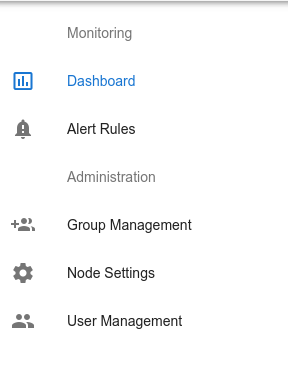
\includegraphics[width=.4\linewidth]{prototype/menu.png}
  \caption{The Main Menu.}
  \label{dbc}
\end{figure}
\paragraph{User Profile}
To access the User Profile, you have to click on the icon on the top right corner.
Every User has access to their User Profile, where they can change their password and e-mail address.
%Picture of Profile missing%
\paragraph{Alert Notification}
On this page, the User can manage alert rules, e.g. they can change the text/thresholds of an alert notification or change the nodes that an alert notification is assigned to.\\
To avoid false positives due to oscillation, the User is able to smooth aberrations. Therefore, it shall be possible to set the acceptable number of threshold violations for a certain period of time. If this number is exceeded, an Alert Notification is sent.
%Picture of Alert page missing%
\paragraph{Alert Rules and Oscillation Handling}. \\
Author: Benedikt Holler | Reviewer: Martin Binder \\ \\
Alert rules consist of thresholds for each KPI, and settings for oscillation handling. All users can create Alert Rules for themselves, but can only assign a single rule to any one node they have Read access to. \\
\textbf{Thresholds} are the central value for monitoring. Users shall set the Threshold for each KPI to a value that would raise concern if it is surpassed frequently. Within \textbf{Oscillation Rules}, User can specify how to handle the oscillation of KPIs with three simple configuration options. \\
\textbf{1. Occurrence:} This attribute indicates how often the threshold has to be surpassed in order to trigger the alert. \\
\textbf{2. Time Frame:} This attribute indicates in what time period the occurrences have to take place in order to trigger the alert. \\
\textbf{3. Sleep:} This attribute indicates how long after an alert is sent it will take before another trigger will occur again. \\
\paragraph{Group Management}
Only privileged Users can access this page. On this page, the privileged User finds a list of User Groups they are in. They can add and remove Users from those Groups.
The Administrator has an overview of all User Groups, and can add or remove Nodes from User Groups.
\paragraph{Node Management}
Similar to Group Management, only privileged Users have access to this page. Privileged Users can change the KPI send interval of nodes which are assigned to their User Groups.
Administrators see all Nodes, and can change their names.
%Picture of Node Management page missing%
\paragraph{User Management}
An Administrator can create/delete/edit other users, for instance giving an user privileged rights.
%Picture of User Management page missing%
\paragraph{Logout}
After a click on logout, the user session is destroyed and the User is redirected to the login
screen. To access the EMS again, the User must re-authenticate.
\subsection{Components}
As it is shown if Fig. \ref{fecomp}, the FE consists of three modules: layouts, pages and 
components.
\begin{figure}[!h]
	\centering
	\includegraphics[width=15cm]{architecture/s03_hams_fe-components.pdf}
	\caption{Rough overview over FE component architecture.}
	\label{fecomp}
\end{figure}
\section{Backend}
% ----------------------------------------- %
Author: Simon Sch\"onberer | Reviewer: Martin Binder\\  \\
The Backend is based on the good old three-tier-architecture and will make use of a few specific
design pattern where applicable.
\subsection{Technologies}
The Backend is built on top of the well known Spring Framework. In particular, we will use
\emph{Spring Boot}, which comes with \emph{Spring Core} and an embedded Tomcat server. This
allows the application to be packaged as an executable JAR (Java ARchive) rather than a
WAR (Web Application Archive). This JAR file is executable by itself due to the embedded tomcat
server. Note that it is also possible to pack the application as WAR, but to prevent confusions
we will stick with JAR.
For the main part of our API via HTTPS, \emph{Spring Web} is needed in order to build the
required controllers. For reactive WSS connections we also need the \emph{Spring Websocket}
extension. For server-side validation, Spring Web already comes with \emph{Spring Validation}.
In order to persist our application's data, we will make use of \emph{Spring Data JPA} to 
access our \emph{JPA} based domain model and use \emph{Hibernate} as persistence provider.
To secure our application we will use \emph{Spring Security} and augment it with
\emph{jwt-security}, a less well known approach to JSON Web Tokens which is tailored to the
use with Spring Security. As we have got to know it as very stable and working out of the
box from previous projects, we do not expect any risk from that decision.
\emph{Spring Mail} will be necessary to send notification messages, and to tackle
cross-cutting-concerns \emph{Spring AOP} (based on \emph{AspectJ}) will be used.
To make our developers' lives easier and our code more readable, we will employ \emph{Project Lombok}
as annotation preprocessor. It enables us to replace tons of boilerplate code like getters,
setters, standard constructors and many more things by simple annotations. Even complex scenarios
like Spring's autowired annotation on a generated constructor are easily possible.
\subsection{Structure}
\begin{figure}[h]
	\centering
	\includegraphics[width=7cm]{architecture/3tier.pdf}
	\caption{3-tier architecture with communication flow}
	\label{3tier}
\end{figure}
\paragraph{Representation Tier.} The controller-classes in this tier are responsible for the
Backend's communication with the outside world. In particular these controllers provide the
entry points for our HTTPS endpoints and WSS/STOMP message mappings as well as the methods to
publish to STOMP topics.
As for HTTPS endpoints, there is nothing special, just every method gets one mapping to a
certain request route. That method calls the appropriate service method subsequently. For
STOMP messaging it is a bit more tricky: Message mappings are not different to HTTPS endpoints,
but we also need to publish to certain topics when some actions occur. In order to achieve
this reactivity, the concerned controllers register with particular services as observers,
in order to receive notifications whenever a relevant action is done.
\paragraph{Business Logic Tier.} The business logic tier (also referred to as service layer)
provides the logical core of our application's functionalities. Every service fulfills an as
accurately as possible defined purpose and has a well defined interface which is available to
the controllers. As for observing controllers, the interfaces also include those methods
that allow observer registration.
\paragraph{Persistence Tier.} The persistence tier allows loading and persisting the data
our application operates on. Therefore it heavily relies on the domain model.
\paragraph{} Figure \ref{beclass} shows an overview.
\begin{figure}[!h]
	\centering
	\includegraphics[width=\linewidth]{uml/class/s02_hams_be-classes.pdf}
	\caption{Specification of BE classes. \\ High resolution PDF in appendix.}
	\label{beclass}
\end{figure}
\subsection{API}
\label{api}
Author: Martin Binder | Review: Benedikt Holler
\subsubsection{FE -- BE: User Management HTTPS}
\begin{tabularx}{12cm}{l|l}
	Path & \url{/users} \\\hline
	Request Method & POST \\\hline
	Description & Create a new User.
\end{tabularx}
\\
\\ \\
\begin{tabularx}{12cm}{l|l}
	Path & \url{/users} \\\hline
	Request Method & GET \\\hline
	Description & Get all User.
\end{tabularx}
\\
\\ \\
\begin{tabularx}{12cm}{l|l}
	Path & \url{/users/:id} \\\hline
	Request Method & GET \\\hline
	Description & Get a specific User.
\end{tabularx}
\\
\\ \\
\begin{tabularx}{12cm}{l|l}
	Path & \url{/users/:id} \\\hline
	Request Method & PUT  \\\hline
	Description & Edit an existing User.
\end{tabularx}
\\
\\ \\
\begin{tabularx}{12cm}{l|l}
	Path & \url{/users/:id} \\\hline
	Request Method & DELETE \\\hline
	Description & Delete a specific User.
\end{tabularx}
\\
\\ \\
\subsubsection{FE -- BE: User Groups HTTPS}
\begin{tabularx}{12cm}{l|l}
	Path & \url{/usergroups} \\\hline
	Request Method & POST \\\hline
	Description & Create a new user-group.
\end{tabularx}
\\
\\ \\
\begin{tabularx}{12cm}{l|l}
	Path & \url{/usergroups} \\\hline
	Request Method & GET \\\hline
	Description & Get all user-groups.
\end{tabularx}
\\
\\ \\
\begin{tabularx}{12cm}{l|l}
	Path & \url{/usergroups/:id} \\\hline
	Request Method & GET \\\hline
	Description & Get a specific user-group.
\end{tabularx}
\\
\\ \\
\begin{tabularx}{12cm}{l|l}
	Path & \url{/usergroups/:id} \\\hline
	Request Method & PUT  \\\hline
	Description & Edit an existing user-group.
\end{tabularx}
\\
\\ \\
\begin{tabularx}{12cm}{l|l}
	Path & \url{/users/:id} \\\hline
	Request Method & DELETE \\\hline
	Description & Delete a specific user-group.
\end{tabularx}
\\
\\ \\
\subsubsection{FE -- BE: Nodes HTTPS}
\begin{tabularx}{12cm}{l|l}
	Path & \url{/nodes} \\\hline
	Request Method & GET \\\hline
	Description & Get a List of Nodes.
\end{tabularx}
\\
\\ \\
\begin{tabularx}{12cm}{l|l}
	Path & \url{/nodes/:id} \\\hline
	Request Method & GET \\\hline
	Description & Get a specific Node.
\end{tabularx}
\\
\\ \\
\begin{tabularx}{12cm}{l|l}
	Path & \url{/nodes} \\\hline
	Request Method & PUT \\\hline
	Description & Update a specific Node.
\end{tabularx}
\\
\\ \\
\begin{tabularx}{12cm}{l|l}
	Path & \url{/node/:id} \\\hline
	Request Method & Delete \\\hline
	Description & Delete a specific Node.
\end{tabularx}
\\
\\ \\
\subsubsection{FE -- BE: Alert Configuration HTTPS}
\begin{tabularx}{12cm}{l|l}
	Path & \url{/alerts} \\\hline
	Request Method & POST \\\hline
	Description & Create an Alert Configuration.
\end{tabularx}
\\
\\ \\
\begin{tabularx}{12cm}{l|l}
	Path & \url{/alerts} \\\hline
	Request Method & GET \\\hline
	Description & Get a List of all Alert Configurations.
\end{tabularx}
\\
\\ \\
\begin{tabularx}{12cm}{l|l}
	Path & \url{/alerts/:id} \\\hline
	Request Method & GET \\\hline
	Description & Get a specific Alert Configuration.
\end{tabularx}
\\
\\ \\
\begin{tabularx}{12cm}{l|l}
	Path & \url{/alerts} \\\hline
	Request Method & PUT \\\hline
	Description & Update an Alert Configuration.
\end{tabularx}
\\
\\ \\
\begin{tabularx}{12cm}{l|l}
	Path & \url{/alerts/:id} \\\hline
	Request Method & DELETE \\\hline
	Description & Delete a specific Alert Configuration.
\end{tabularx}
\\
\\ \\
\subsubsection{FE -- BE: Server Settings HTTPS}
\begin{tabularx}{12cm}{l|l}
	Path & \url{/settings} \\\hline
	Request Method & GET \\\hline
	Description & Get the Server Settings.
\end{tabularx}
\\
\\ \\
\begin{tabularx}{12cm}{l|l}
	Path & \url{/settings} \\\hline
	Request Method & PUT \\\hline
	Description & Update the Server Settings.
\end{tabularx}
\subsubsection{FE -- BE: STOMP OVER WSS}
\begin{tabularx}{12cm}{l|l}
	Path & \url{/topics/dashboardConfiguration} \\\hline
	Request Method & SUBSCRIBE \\\hline
	Description & FE subscribes to topic.
\end{tabularx}
\\
\\ \\
\begin{tabularx}{12cm}{l|l}
	Path & \url{/topics/dashboardConfiguration} \\\hline
	Request Method & UNSUBSCRIBE \\\hline
	Description & FE cancels the connection. 
\end{tabularx}
\\
\\ \\
\subsubsection{MC -- BE: Nodes HTTPS}
\begin{tabularx}{12cm}{l|l}
	Path & \url{/mc/register} \\\hline
	Request Method & POST \\\hline
	Description & MC registers with the BE. 
\end{tabularx}
\\
\\ \\
\subsubsection{MC -- BE: Nodes WSS}
\begin{tabularx}{12cm}{l|l}
	Path & \url{/mc/kpi/} \\\hline
	Request Method & SEND \\\hline
	Description & MC sends a set of KPIs to the BE. 
\end{tabularx}
\section{Monitoring Client}
% ----------------------------------------- %
Author: Korbinian Simonis | Reviewer: Simon Sch\"onberer \\ \\
In this section we describe the Monitoring Client, in particular the technology used, the architecture and the communication with the BE.
\subsection{Technology}
Our MC will be written in Python, since it's a very powerful yet easily understandable language. Python's design philosophy emphasizes code readability and simplicity, which results in a very intuitive way of programming. As Python is an extensible programing language, there are plenty of modules, providing additional functionalities to use. \\
In concrete, we decided to use \textbf{Python3}, since it is under active development, unlike Python2. This means that all recent standard library improvements, for example, are only available by default in Python 3.x. \\
In order to implement the desired functionality, a variety of standard libraries will be needed, such as \textit{sys}, \textit{os}, \textit{http}, \textit{json}, \textit{subprocess}, \textit{multiprocessing} but also some custom libraries like \textit{psutil}, which will be the core module for our KPI collecting. \\
\textbf{psutil} is a cross-platform library mainly used for monitoring, profiling, limiting resources and for managing processes. It provides information on running processes and system utilization (CPU, memory, disks, network, sensors) and therefore already implements many functionalities offered by UNIX command line tools such as netstat, ps, lsof and top. Psutil supports currently all common platforms like Linux, Windows, macOS, FreeBSD and Sun Solaris. \\
\textbf{multiprocessing} is a module that, like threading, can be used to parallelize concurrent operations. It provides true system process without shared memory and is therefore 'real' parallel. Threading, on the other hand, creates thread objects, which runs concurrently within the same process and share memory. In CPython, due to the Global Interpreter Lock, only one thread can execute Python code at once, so threading offers no 'real' parallelism. Also, the handling of processes has proved to be less complicated, so we have decided to use multiprocessing.
\subsection{Architecture}
Since we will be using Python and the required functionalities are straightforward, there is no need for complicated design patterns, which is why we plan on following the \textbf{KISS-principle} (Keep it simple, stupid) for the architecture of our MC.  
But for the sake of clarity and to facilitate maintenance, we will segment our script in a main script and several modules.
\paragraph{modules}: We plan on providing an extra module for every KPI and the energy measurement, which can be imported in our main script. A Python module is a file containing definitions and statements. 
\paragraph{main}: We plan on utilizing multiprocessing to ensure maximum responsiveness to possible configuration changes, such as the sending interval of a node. In concrete, we want to use a process for the KPI collecting/sending (collector) and one for the process managing (manager). In the collector, the imported KPI functions are executed in a while-loop and at the end of every loop, the KPI-Package (JSON format) is sent to the BE. The manager starts/stops the collector and listens to changes from the BE.
\begin{figure}[H]
	\centering
	\includegraphics[width=13cm]{uml/class/mc_class_diagram_new.pdf}
	\caption{Class diagram of our MC}
	\label{class_mc}
\end{figure}
\subsection{Communication}
The only communication the MC needs to provide, is to the BE.
Here, we have to cover three different scenarios. \\
On one hand, the registration of a client on the backend, on the other hand sending of KPI packages to the BE and receiving of configuration changes from the BE.
For registration, we will use HTTPS as shown in \textbf{MC | BE: Nodes HTTPS} in Section \ref{api}. \\
For the other two connections, we will use websockets (Section \ref{websockets}). The MC subscribes to a topic on the BE and receives configuration changes over WSS (websocket secure). Since websockets provide a two-way interactive communication session, the collector can also use this connection to send KPI packages (see Section \ref{api}, \textbf{MC | BE: Nodes WSS}).
%---------------------------------------%
\section{Data Transfer Objects}
Author: Martin Binder | Reviewer: Andreas M\"uller\\ \\
It's important to reduce the traffic between components and achieve a cheap communication with as little API calls as possible. In order to accomplish those goals, we use Data Transfer Objects, or \textbf{DTOs} for short.
\subsection{DashboardConfigDTO}
The DashboardConfigDTO is used to send requests from the Client to the Server demanding a certain data set. The DTO consists of information about the selected node and the time interval the User has chosen.  
\begin{figure}[H]
	\centering
	\includegraphics[width=10cm]{DTO/DashboardConfigDTO.pdf}
	\label{dashboardConfigDTO}
\end{figure}
\newpage
\subsection{AlertRuleDTO}
The composition of Alert Rules can lead to an increase in traffic between Client and Server. To prevent this we use AlertRuleDTOs which are a compilation of \textbf{AlertRule}, \textbf{configures}, \textbf{User},  \textbf{observes}, \textbf{KPI}, \textbf{typeOf}, \textbf{Record}, \textbf{triggers}, \textbf{Notification} (See Figure \ref{er}). When creating, assigning, removing or deleting Alert Rules all of those entities are prone to change. To reduce the amount of calls and requested packages the essential information to identify the entities and process the request is stored in a DTO.  
\begin{figure}[H]
	\centering
	\includegraphics[width=10cm]{DTO/AR_DTO.pdf}
	\label{alertRuleDTO}
\end{figure}
\newpage
\subsection{UserGroupDTO}
In order to represent User Groups, multiple data sets have to be requested from the Server, including \textbf{User}, \textbf{UserGroups}, \textbf{Nodes}, \textbf{isPartOf}, \textbf{assignedTo}(See Figure \ref{er}) . For a UserGroup with multiple Nodes assigned to it and multiple Users as members, this can lead to a high amount of traffic and API requests. With the UserGroupDTO we create a single object which can be requested by the Client and which contains all necessary information to process the requests.
\begin{figure}[H]
	\centering
	\includegraphics[width=10cm]{DTO/UG_DTO.pdf}
	\label{userGroupDTO}
\end{figure}
\subsection{MCKpiPackageDTO}
The MC sends KPIs consisting of a \emph{name} and \emph{value}, along with identifying information \emph{nodeId} and \emph{timestamp} to the Server. In order to easily process those, we use MCKpiPackageDTOs with an eye on future scaling and a generic approach on how to handle upcoming changes in the sent KPI set the design of the DTO allows to easily add KPI sets without any changes to MCKpiPachageDTO. 
\begin{figure}[H]
	\centering
	\includegraphics[width=10cm]{DTO/MCKpiPackageDTO.pdf}
	\label{trivialDTO}
\end{figure}
% ================================================================ %

% ----------------------------------------- %

\includepdf[page={1}, angle=90, scale=0.55, pagecommand={\chapter{Data Model} \section{Entity Relationship Model}}]{er/er.pdf}
\label{er}

\section{Database Schema}
Author: ER \& DB Schema Benedikt Holler | Reviewer: Korbinian Simonis\\ \\
% ----------------------------------------- %
ER High resolution PDF in appendix. \\
From the ER model above, we deduced the following Database Schema. \\ 
Attributes written in \textbf{bold} constitute that table's Primary Key. Attributes in \emph{italics} are Foreign Keys, and the attribute in the foreign table they reference is in brackets.\\ \\
\begin{tabularx}{15cm}{l|X}
	\hline 
\textbf{Table Name}	& \textbf{Attributes} \\ 
	\hline 
Node	&\textbf{ID:Long}, Name:String,  Send\_Interval:Long  \\ 
	\hline 
Record	& \textbf{ID:Long}, Timestamp:Long, Value:Float, \emph{Type:Long(KPIs.ID)}, \emph{SentBy:Long(Node.ID)} \\ 	
	\hline
KPI & \textbf{ID:Long}, Name:String, Unit:String \\
	\hline
User	& \textbf{ID:Long}, E-Mail:String, Name:String, Password:String, IsAdmin:Boolean, IsPrivileged:Boolean \\ 
	\hline 
User\_Group	&\textbf{ID:Long}, Name:String  \\ 
	\hline 
Alert\_Rule	&\textbf{ID:Long}, Name:String, Oscillation\_Occurrence\_Count:Long, Oscillation\_Time:Long, Sleep\_Time:Long,  \emph{ConfiguredBy:Long(Users.ID)}  \\ 
	\hline 
Notification	&\textbf{ID:Long}, Timestamp:Long, Text:String, \emph{Recipient:Long(Users.ID)} \\
\hline 
Rule\_Designation & \textbf{\emph{Rule:Long(Alert\_Rules:ID)}}, \textbf{\emph{Node:Long(Nodes.ID)}}, \textbf{\emph{KPI:Long(KPIs.ID)}}, Lower\_Or\_Equal:Boolean, Threshold: Float \\ 
	\hline 
Node\_Assignment	&\textbf{\emph{Node:Long(Nodes.ID)}}, \textbf{\emph{User\_Group:Long(User\_Groups.ID)}},   \\ 
	\hline 
Group\_Membership	&\textbf{\emph{User:Long(Users.ID)}}, \textbf{\emph{Group:Long(User\_Groups.ID)}}  \\ 
	\hline 
\end{tabularx} 
\section{Domain Model}
% ----------------------------------------- %
Author: Korbinian Simonis | Reviewer: Simon Sch\"onberer \\ \\
In this section we provide the jpa domain class diagram (\ref{class_domain}). \\
In order to keep it simple and clear, the respective getter and setter methods of the individual attributes are not depicted in the diagram. Also some relations needs additional explanations, for instance User and UserGroup. It shall be possible to create a User with no group assignment, analogously it shall be possible to create an UserGroup with no Users in it. The reasons for that are not only the easier implementation, but also security aspects. For example, if a user is absent for a longer period of time (parental leave, long vacation etc.), we do not want to have to deactivate the account, but neither allow unused accounts with possibly privileged rights in the system. A practicable solution here is to simply remove the user from their groups and thereby deprive them of relevant rights on nodes.
Furthermore, such an approach is not uncommon and is handled this way in a variety of applications. 
\begin{figure}[h!]
	\centering
	\includegraphics[scale=0.5, angle=270]{uml/class/s03_hams_be-domainclasses_new}
	\caption{Domain class diagram}
	\label{class_domain}
\end{figure}
\chapter{Control Flow}
% ================================================================ %
Author: Martin Binder | Review: Korbinian Simonis
\section{Authentication}
Author: Korbinian Simonis | Review: Andreas M\"uller  \\ \\
For Authentication, we use \textbf{JSON Web Token} (JWT), which is an open standard (RFC 7519) that defines a compact and self-contained way for securely transmitting information between parties as a JSON object. To ensure trust, JWTs can be signed using signature algorithms (HMAC) or a public/private key pair using RSA or ECDSA. Since the signing only verifies the integrity of the claims contained within a request, we send JWTs only over HTTPS connections, to prevent unauthorized users from stealing them. \\
Furthermore, there are already Spring Security Addons for JWT, which provides a simple way to integrate JWT into a spring boot application. \\
For instance \fbox{\parbox{9cm}{HTTPS://github.com/bratkartoffel/security-jwt-examples}}.\\
%\begin{figure}[h!]
%	\centering
%	\includegraphics[width=12cm]{uml/sequence/s03_hams_sequence_auth.pdf}
%	\caption{Sequence diagram: Authentication}
%	\label{seq_auth}
%\end{figure}
\noindent Figure \ref{alertSequence} shows an example of the authentication process using cookies and refresh token.
At the start, the User sends a POST request containing his credentials to the Backend. If the credentials are valid, the JWT library in the backend responds with 200 OK and provides an \textbf{AccessToken} and a \textbf{RefreshToken} stored in a cookie. 
\paragraph{Access-Token} carry the necessary information to access a resource directly, that means when a client passes an access token to a server managing a resource, the server can use the information contained in the token to decide whether the client is authorized or not. Access tokens usually have an expiration date and are short-lived.
\paragraph{Refresh-Token} is used to generate a new access token. If the access token expires, the user would have to authenticate again to get a new access token. With a refresh token, this step can be skipped and the User can request to the API to get a new access token that allows him to continue accessing the requested data. Refresh-Token are rather long-lived and can be blacklisted by a server to prevent security issues. \\

\noindent As long an Access-Token is valid, an User can access data as shown in Figure \ref{alertSequence} with the GET /ham request. If the Access-Token expires, the User needs the Refresh-Token in order to get a new Access-Token.


% ----------------------------------------- %
\section{STOMP over Websocket} \label{websockets}
For the connection between FE and BE and also between MC and BE we decided to use STOMP over WebSocket to enable a near real time and  pushed-by-the-server continuous connection.
\subsection{Websocket}
To satisfy the demands of the communication architecture between the FE, BE and MC, where the BE pushes updates without the FE explicit request (always when they become available), we chose WebSocket as the continuous connection to enable the desired behavior. With WebSocket data that is received by the BE (i.e. new sets of KPIs) can be pushed to the FE, thus enabling an efficient full duplex communication. In the same way, configuration changes regarding the MCs are pushed to the MCs by the BE as fast as the Backend becomes aware of them. Another major advantage is the compared small package size and low latency that WebSocket protocol provides which saves resources and leads in smoother scaling.
\subsection{Simple(Streaming) Test Oriented Messaging Protocol}
Author: Martin Binder | Review: Simon Schönberger\\ \\
STOMP is an implementation-agnostic simple and lightweight messaging protocol. We decided
to use it in order to add stronger semantics on top of the raw WS-frames. It provides a few
operations like \texttt{CONNECT, DISCONNECT, SUBSCRIBE, UNSUBSCRIBE, SEND} and a few others
which allow clients to interact with message brokers.
STOMP offers a simple lightweight solution to handle the communication between client and server. With the focus on messaging semantics especially the STOMP frames and the key/value pairs used in STOMP messages. Those allow an easy implementable solution to how new KPIs are sent and can easily be understood by the FE and facilitates continuous updates.
After an initial handshake, clients can subscribe themselves to certain topics and
receive data whenever the topic gets updated by the message broker. They are also able to
send messages to the message broker.
In our application, the BE will act as a message broker for FE and MCs. The FE subscribes to
a topic, to which updates to the current Dashboard get published. Each MC subscribes to
a topic, on which configuration changes will be pushed. Vice versa the MCs send messages
with KPI updates to the BE.
% ----------------------------------------- %
\section{E-mail - Notifications}
E-mail alerts are sent using the JavaMailSender interface for which spring boot provides an auto-configuration that enables a quick and easy implementation. With some minor setting changes a Bean can be configured with an Email address that will be used to send notifications to Users in case the configured threshold for a node is exceeded. As for the development phase a Google SMTP server will be used until an usable Email address is provided by the customer.
\pagebreak
\section{Sequence diagram}
\subsection{Login}
Author:  Andreas M\"uller |
Reviewer: Simon Sch\"onberger\\ \\
% ----------------------------------------- %
The following sequence diagram describes the use-case "Login". \\
A User enter their credentials in the login page. The BE checks the information and creates JWTs.
\\ \\
\begin{figure}[h]
	\centering
	\includegraphics[width=15cm]{uml/sequence/s03_hams_sequence_login.pdf}
	\caption{Sequence diagram: Login}
	\label{alertSequence}
\end{figure}
\pagebreak
\subsection{Login Fail}
Author:  Andreas M\"uller |
Reviewer: Simon Sch\"onberger\\ \\
This sequence diagram describes the same use-case as the previous one,
but the user is not authorized.
\\ \\
\begin{figure}[h]
	\centering
	\includegraphics[width=15cm]{uml/sequence/s03_hams_sequence_login_fail.pdf}
	\caption{Sequence diagram: Login Fail}
	\label{failSequence}
\end{figure}
\pagebreak
\subsection{Node Management}
% ----------------------------------------- %
Author:  Andreas M\"uller |
Reviewer: Simon Sch\"onberger\\ \\
In this sequence the Administrator deletes a Node.
To delete a Node the Administrator navigates to the Node Management page where they get an overview of all Nodes. After selecting a Node the Administrator delete the Node.
The changes will be saved, and displayed on the FE.
After this, the Administrator has to remove the MC from the node.
\\ \\
\begin{figure}[h]
	\centering
	\includegraphics[width=13cm]{uml/sequence/s03_hams_sequence_node_management.pdf}
	\caption{Sequence diagram: Privileged User edits Node}
	\label{editUserSequence}
\end{figure}
\pagebreak
\subsection{User Managemenet}
% ----------------------------------------- %
Author:  Andreas M\"uller |
Reviewer: Simon Sch\"onberger\\ \\
In this sequence, the Administrator changes the username. 
To change the name of an User, the Administrator navigates to the User Management page, where they get an overview of all Users. After selecting an User, the Administrator can edit the User e.g. username.
The changes will be saved and displayed on the FE.
\\ \\
\begin{figure}[h]
	\centering
	\includegraphics[width=13cm]{uml/sequence/s03_hams_sequence_user_management.pdf}
	\caption{Sequence diagram: Administrator edits User}
	\label{editNodeSequence}
\end{figure}
\pagebreak
\subsection{Alert Trigger}
% ----------------------------------------- %
Author:  Andreas M\"uller |
Reviewer: Simon Sch\"onberger\\ \\
The following sequence diagram shows what happens when a User receives an Alert Notification, e.g. e-mail. \\
It all starts when the MC sends KPIs to the BE. The BE compares received KPIs with the Alert Rule they have from the Database.
In this example at least one KPI surpasses its Threshold, so the BE sends an Alert Notification to the User.
\\ \\
\begin{figure}[h]
	\centering
	\includegraphics[width=15cm]{uml/sequence/s03_hams_sequence_alert_trigger.pdf}
	\caption{Sequence diagram: Alert Rule gets triggered}
	\label{alertTriggerSequence}
\end{figure}
\pagebreak
\subsection{MC installation and registration}
% ----------------------------------------- %
Author:  Korbinian Simonis |
Reviewer: Simon Sch\"onberger\\ \\
This sequence diagram shows the installation and registration of the MC on a new node.\\
The first step to install the MC is to request a token, which will be needed for the later registration of the MC at the BE. The Admin can request this token in the FE. In the background, a request is sent to the BE, which then transmits the token to the FE. \\
After that, the Administrator copies the package (e.g. a zip file) to the node, unzips it and executes the install script with the token as parameter. The MC then installs itself and sends a registration request (with token) to the BE. If the token is valid, the BE accepts the registration and transmits the data of the node to the database. The MC is now registered.
\\ \\
\begin{figure}[h]
	\centering
	\includegraphics[width=15cm]{uml/sequence/s03_hams_sequence_mc_instal_reg.pdf}
	\caption{Sequence diagram: Administrator installs MC}
	\label{mcInstallationSequence}
\end{figure}
\pagebreak
\subsection{MC update send interval}
% ----------------------------------------- %
Author:  Korbinian Simonis |
Reviewer: Simon Sch\"onberger\\ \\
This sequence diagram shows how a change of the send interval is processed. \\
An Administrator / Super-user can change the send interval of a node in the FE. This change request is transmitted to the BE and receives in response just an acknowledgment, since at this time no statement can be made whether the change can be processed or not.
The BE then forwards the change request to the MC of the affected node, which then immediately begins to apply the new send interval.
\\ \\
\begin{figure}[h]
	\centering
	\includegraphics[width=15cm]{uml/sequence/s03_hams_sequence_mc_change.pdf}
	\caption{Sequence diagram: Administrator changes send interval of MC}
	\label{mcChangeIntervalSequence}
\end{figure}
\end{document}
